% CHAPTER SLIDE
\cscschapter{Scaling Up : Thread Blocks}

%%%%%%%%%%%%%%%%%%%%%%%%%%%%%%%%%%%%%%%%%%%%
\begin{frame}[fragile]{Thread Blocks}
%%%%%%%%%%%%%%%%%%%%%%%%%%%%%%%%%%%%%%%%%%%%
    \begin{info}{}
        In the \axpy exercises we were limitted to 1024 threads for a kernel launch
        \begin{itemize}
            \item But GPUs are about \emph{massive parallelism}
        \end{itemize}
    \end{info}

    \begin{info}{thread blocks and grids}
        \begin{itemize}
            \item Kernels are executed in groups of threads called \emph{thread blocks}
            \item the launch configuration \lst{axpy<<<grid_dim, block_dim>>>(...)}
            \begin{itemize}
                \item launch a \emph{grid} of \lst{grid_dim} \emph{blocks}
                \item each \emph{block} has \lst{block_dim} \emph{threads}
                \item for a total of \lst{grid_dim}$\times$\lst{block_dim} threads
            \end{itemize}
            \item so far we have been launching one thread block \lst{axpy<<1, n>>(...)}
        \end{itemize}
    \end{info}

\end{frame}

%%%%%%%%%%%%%%%%%%%%%%%%%%%%%%%%%%%%%%%%%%%%
\begin{frame}[fragile]{Thread Blocks : motivation behind blocks and grids}
%%%%%%%%%%%%%%%%%%%%%%%%%%%%%%%%%%%%%%%%%%%%
    this might be split into 3-4 slides, each slide with a picture and 1-2 points per slide
    \begin{info}{why the additional complexity of grids+blocks+threads?}
        \begin{itemize}
            \item threads in a block can synchronize and share resources
            \item this does not scale past a certain point
            \item GPU has 14 streaming multiprocessors (SMXs)
            \item each SMX has 192 CUDA cores, and can run 2028 threads sumultaneously
            \item threads in a block all run on the same SMX (share resources like shared memory)
            \item break the work into blocks, which are distributed over the different SMXs
        \end{itemize}
    \end{info}
\end{frame}

%%%%%%%%%%%%%%%%%%%%%%%%%%%%%%%%%%%%%%%%%%%%
\begin{frame}[fragile]{Mapping Kernels to Hardware}
%%%%%%%%%%%%%%%%%%%%%%%%%%%%%%%%%%%%%%%%%%%%
\begin{center}
\vspace{-0.75cm}
\begin{tabular}{|c|m{4cm}|m{5cm}|}
    \cline{1-2}
        concept & hardware &  \multicolumn{1}{c}{} \\
    \hline
        thread &
        \begin{minipage}{4cm}
            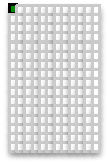
\includegraphics[width=0.3\textwidth]{./images/core.pdf}
        \end{minipage} &
        \footnotesize
        \begin{itemize}
            \item each thread executed on one core
        \end{itemize} \\
    \hline
        block &
        \begin{minipage}{4cm}
            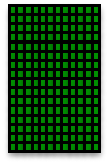
\includegraphics[width=0.3\textwidth]{./images/smx.pdf}
        \end{minipage} &
        \footnotesize
        \begin{itemize}
            \item block executed on 1 SMX
            \item multiple blocks per SMX if sufficient resources
            \item threads in a block share SMX resources
        \end{itemize} \\
    \hline
        grid &
        \begin{minipage}{4cm}
            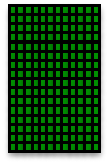
\includegraphics[width=0.3\textwidth]{./images/smx.pdf}
            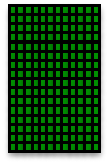
\includegraphics[width=0.3\textwidth]{./images/smx.pdf}
            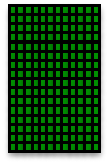
\includegraphics[width=0.3\textwidth]{./images/smx.pdf}
        \end{minipage} &
        \footnotesize
        \begin{itemize}
            \item kernel is executed in grid of blocks
            \item blocks distributed over SMXs
            \item multiple kernels can run at same time
        \end{itemize} \\
\hline
\end{tabular}
\end{center}
\end{frame}

%%%%%%%%%%%%%%%%%%%%%%%%%%%%%%%%%%%%%%%%%%%%
\begin{frame}[fragile]{Calculating thread indexes}
%%%%%%%%%%%%%%%%%%%%%%%%%%%%%%%%%%%%%%%%%%%%
    All kernels first calculate the index or position 
    \begin{itemize}
        \item In \lst{axpy} we used the \emph{magic variable} \lst{threadIdx.x} for the index $i$
        \item When using multiple blocks, we need more information, which is available in the following \emph{magic variables}:

    \end{itemize}

    \begin{center}
        \begin{tabular}{|l|l|}
            \hline
        \lst{gridDim}   & total number of blocks in the grid \\
        \lst{blockDim}  & number of threads in a thread block \\
        \lst{blockIdx}  & index of block \lst{[0, gridDim-1]} \\
        \lst{threadIdx} & index of thread in thread block \lst{[0, blockDim-1]} \\
            \hline
        \end{tabular}
    \end{center}
\end{frame}

%%%%%%%%%%%%%%%%%%%%%%%%%%%%%%%%%%%%%%%%%%%%
\begin{frame}[fragile]{Using Thread Blocks}
%%%%%%%%%%%%%%%%%%%%%%%%%%%%%%%%%%%%%%%%%%%%
    \begin{center}
        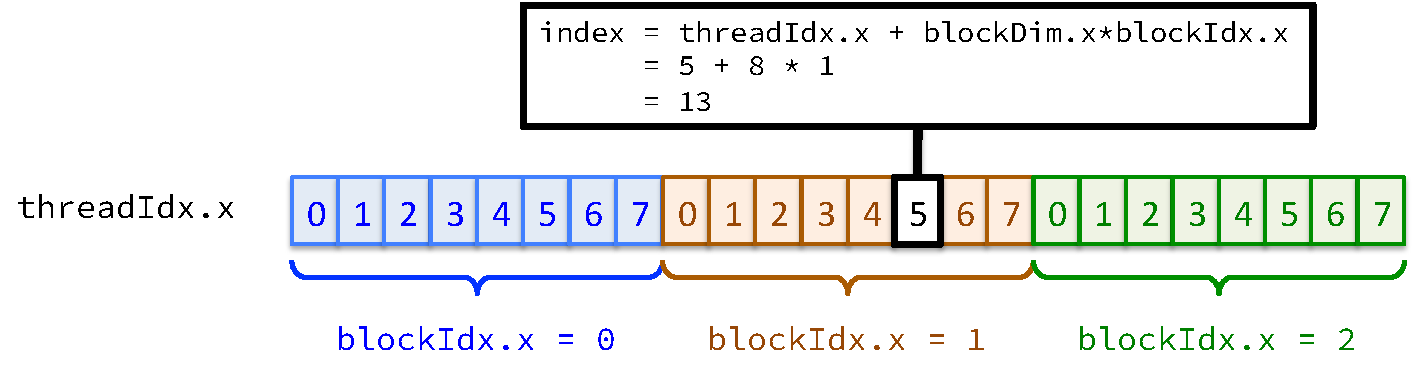
\includegraphics[width=\textwidth]{./images/blocks.pdf}
    \end{center}
\end{frame}

%%%%%%%%%%%%%%%%%%%%%%%%%%%%%%%%%%%%%%%%%%%%
\begin{frame}[fragile]{Practicalities}
%%%%%%%%%%%%%%%%%%%%%%%%%%%%%%%%%%%%%%%%%%%%
    explain how to calculate the number of blocks and threads

    maybe how to optimize this?
\end{frame}


